\documentclass[12pt,letterpaper]{article}

\usepackage[utf8]{inputenc}
\usepackage[T1]{fontenc}
\usepackage[spanish]{babel}
\usepackage[margin=2.54cm]{geometry}
\usepackage{setspace}
\usepackage{titlesec}
\usepackage[hypertexnames=false,bookmarks=false]{hyperref}
\usepackage{helvet}
\usepackage{fancyhdr}
\usepackage{enumitem}
\usepackage{tabularx}
\usepackage{array}
\usepackage{graphicx}
\usepackage{caption}
\usepackage{float}
\usepackage{placeins}

\captionsetup{font=footnotesize,labelfont=bf,justification=centering}
\graphicspath{{docs/images/prototipos/}{images/prototipos/}}

\setlength{\headheight}{15pt}
\renewcommand{\familydefault}{\sfdefault}

\doublespacing
\setlength{\parindent}{1.27cm}
\setlength{\parskip}{0pt}

\pagestyle{fancy}
\fancyhf{}
\rhead{\thepage}
\renewcommand{\headrulewidth}{0pt}

\titleformat{\section}
{\normalfont\bfseries}
{\thesection.}{0.5em}{}

\titleformat{\subsection}
{\normalfont\bfseries}
{\thesubsection.}{0.5em}{}

\hypersetup{
    colorlinks=true,
    linkcolor=black,
    urlcolor=black
}

\renewcommand{\arraystretch}{1.25}
\newcolumntype{Y}{>{\raggedright\arraybackslash}X}
\newcolumntype{B}[1]{>{\bfseries\raggedright\arraybackslash}p{#1}}

\begin{document}

\begin{titlepage}
    \centering

    {\large \textbf{UNIVERSIDAD MAYOR DE SAN SIMON}}\\
    {\large \textbf{FACULTAD DE CIENCIAS Y TECNOLOGIA}}\\
    {\large \textbf{CARRERA DE INGENIERIA INFORMATICA}}\\[0.5cm]

    \rule{\textwidth}{0.5pt}\\[0.5cm]
    {\Large \textbf{Trabajo Final -- Semana 4}}\\[0.3cm]
    {\large \textbf{Prototipo funcional y evaluacion}}\\[0.5cm]
    \rule{\textwidth}{0.5pt}\\[1cm]

    {\large \textbf{Tema}}\\[0.3cm]
    {\large Sistema de control para la distribucion presencial de guias academicas en la Carrera de Fisica}\\[2cm]

    \begin{flushleft}
        \textbf{Integrantes:}\\
        \hspace*{0.5cm}\textbullet\ Jose Daniel Virreira Rufino\\
        \hspace*{0.5cm}\textbullet\ Mairon Henry Fernandez Orellana\\
        \hspace*{0.5cm}\textbullet\ Jonas Vidal Zenzano\\
        \hspace*{0.5cm}\textbullet\ Luis Fernando Cardenas Morales
    \end{flushleft}

    \begin{flushleft}
        \textbf{Grupo:} UXploradores\\
        \textbf{Materia:} Interaccion Humano-Computadora\\
        \textbf{Docente:} Mgr. Corina Flores Villarroel\\
        \textbf{Gestion:} I-2026
    \end{flushleft}

    \vfill

    {\small Cochabamba -- Bolivia}\\
\end{titlepage}

El presente informe corresponde a la Semana 4 del proyecto. En esta etapa se desarrollo el prototipo funcional de media/alta fidelidad y se preparo su evaluacion mediante pruebas de usabilidad y revision heuristica. La prueba con usuarios externos queda planificada para la siguiente iteracion; por ello, este documento presenta el estado funcional del prototipo, una revision heuristica inicial y recomendaciones de mejora antes de aplicar la prueba con otra persona.

\section{Objetivo de la semana}

Desarrollar una version funcional inicial del prototipo y evaluarla para identificar problemas de uso antes de la etapa de correccion.

\section{Prototipo funcional}

El prototipo fue implementado como una aplicacion web conectada a Supabase. Las pantallas principales ya permiten trabajar con datos reales del sistema.

\begin{center}
\begin{tabularx}{\textwidth}{|B{4cm}|Y|}
\hline
Pantalla & Funcionalidad principal \\
\hline
Dashboard & Muestra resumen de stock, cuentas y movimientos recientes. \\
\hline
Registrar entrega & Permite seleccionar guia, cantidad y metodo; descuenta stock y registra movimiento. \\
\hline
Inventario & Presenta stock y movimientos por tipo de guia. \\
\hline
Consulta estudiante & Muestra guia, materia, precio y disponibilidad. \\
\hline
Cuentas & Registra ingresos, salidas y retiros entre cuentas. \\
\hline
Pedidos & Registra llegada de guias y actualiza inventario. \\
\hline
Cierre de caja & Compara montos y stock esperado contra valores contados. \\
\hline
\end{tabularx}
\end{center}

\section{Evidencia del prototipo}

\begin{figure}[H]
    \centering
    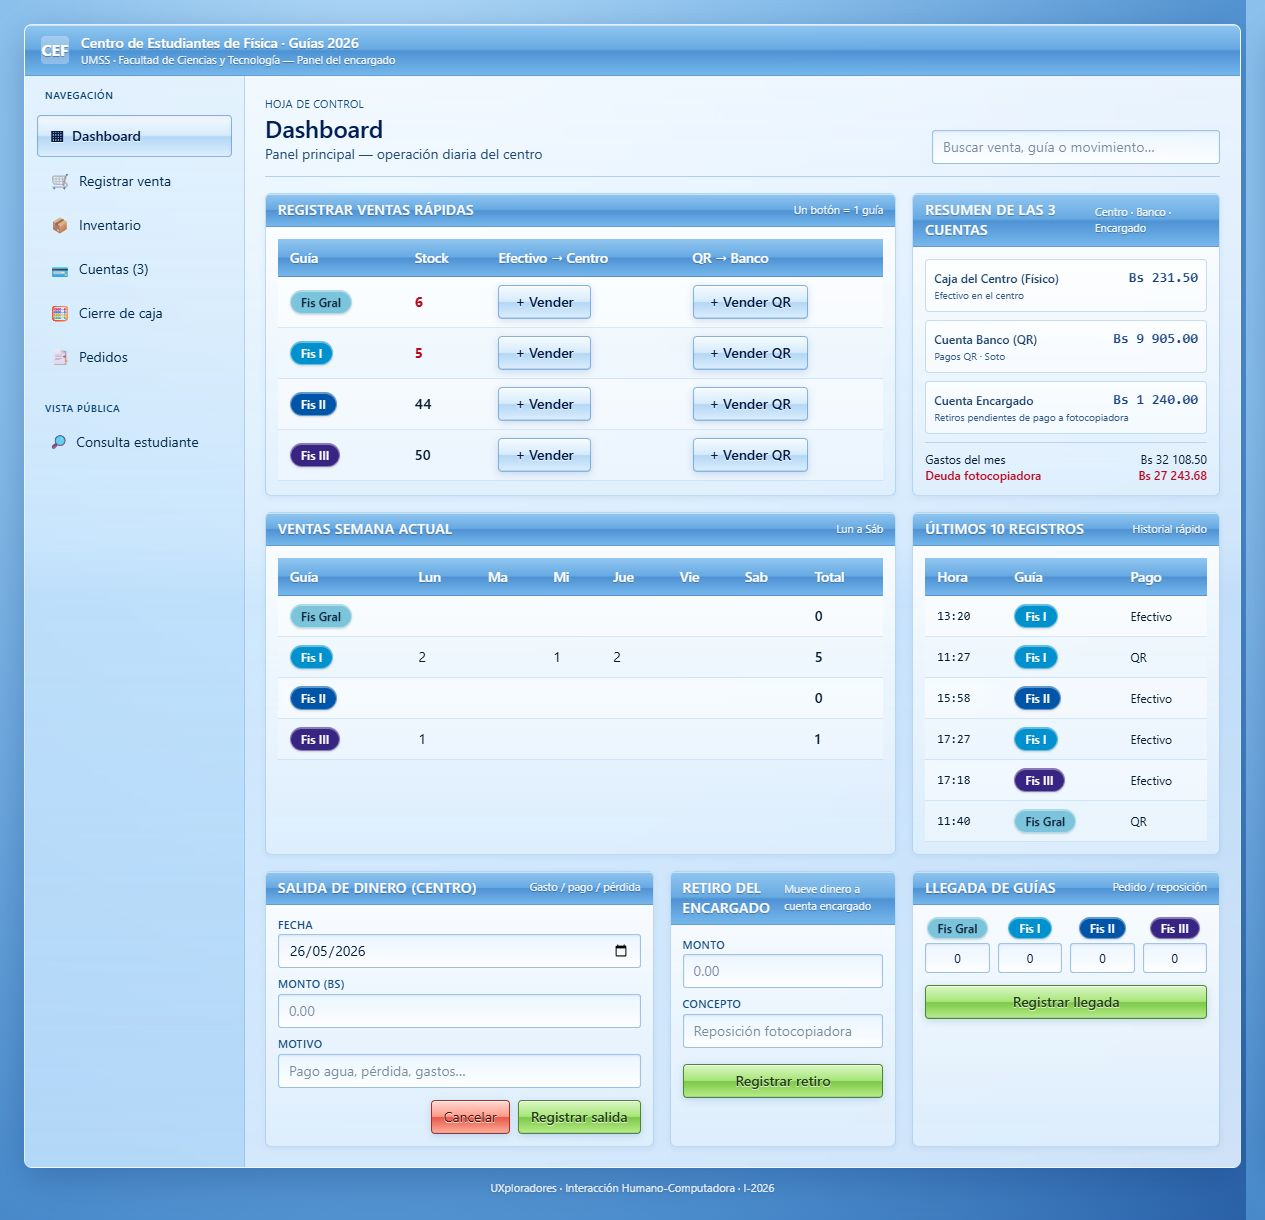
\includegraphics[width=0.9\textwidth,height=0.45\textheight,keepaspectratio]{prototipo_dashboard.png}
    \caption{Dashboard funcional conectado a datos reales.}
\end{figure}

\begin{figure}[H]
    \centering
    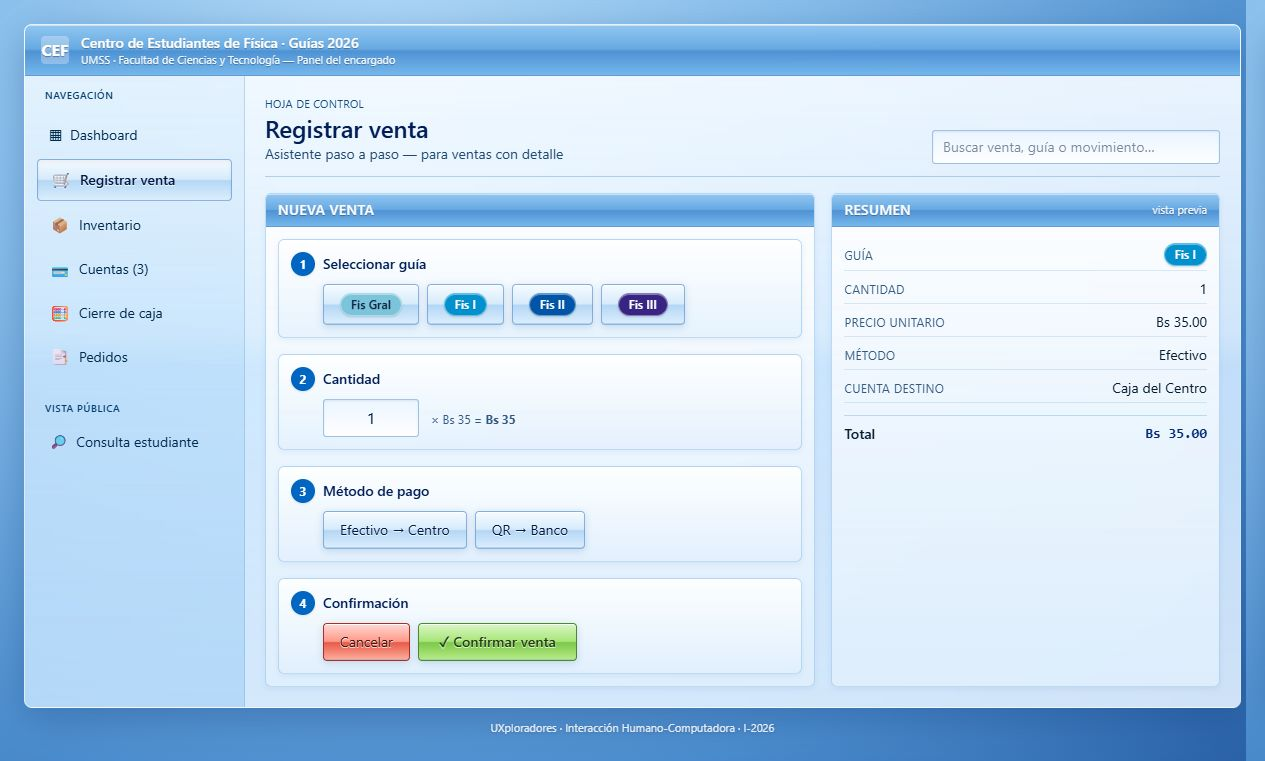
\includegraphics[width=0.9\textwidth,height=0.45\textheight,keepaspectratio]{prototipo_venta.png}
    \caption{Registro de entrega con seleccion de guia, cantidad y metodo.}
\end{figure}

\begin{figure}[H]
    \centering
    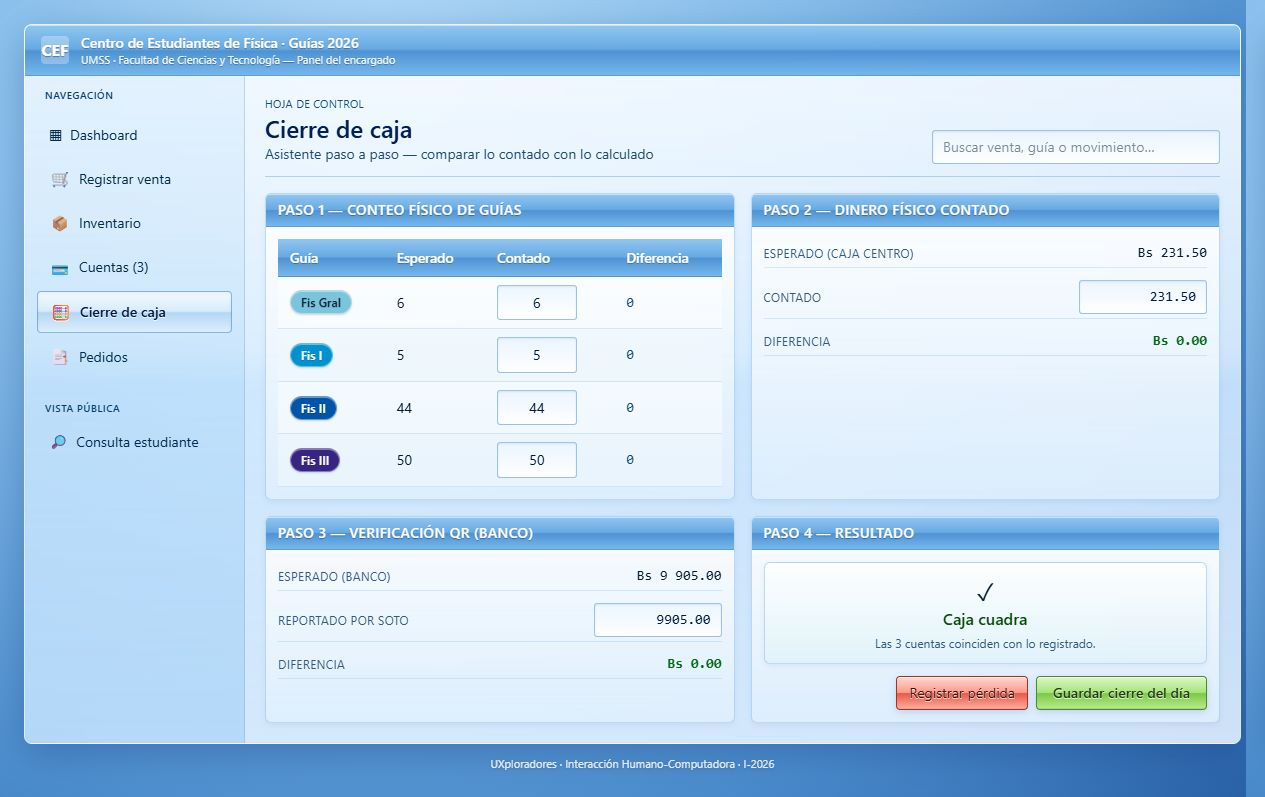
\includegraphics[width=0.9\textwidth,height=0.45\textheight,keepaspectratio]{prototipo_cierre.png}
    \caption{Cierre de caja con comparacion de valores esperados y contados.}
\end{figure}

\FloatBarrier

\section{Prueba de usabilidad planificada}

La prueba de usabilidad se aplicara con usuarios representativos mediante tareas breves. El objetivo sera observar si las acciones principales pueden completarse sin explicacion extensa. Para esta semana se definio el protocolo de evaluacion y las tareas que se usaran durante la prueba.

\begin{center}
\begin{tabularx}{\textwidth}{|B{3cm}|B{3cm}|Y|B{2.4cm}|}
\hline
Participante & Perfil & Tarea evaluada & Resultado \\
\hline
P1 & Encargado & Registrar una entrega de guia. & Por aplicar \\
\hline
P2 & Estudiante & Consultar disponibilidad y precio. & Por aplicar \\
\hline
P3 & Encargado & Revisar cierre o movimiento de cuenta. & Por aplicar \\
\hline
\end{tabularx}
\end{center}

\section{Evaluacion heuristica}

Tambien se realizo una revision rapida del prototipo con criterios de usabilidad. Se priorizaron aspectos visibles durante el uso del sistema.

\begin{center}
\begin{tabularx}{\textwidth}{|B{4cm}|Y|B{2.5cm}|}
\hline
Criterio & Observacion & Severidad \\
\hline
Visibilidad del estado & El sistema muestra estados de carga, error o confirmacion en las pantallas principales. & Baja \\
\hline
Prevencion de errores & Algunas acciones validan cantidad, stock y montos antes de guardar. & Media \\
\hline
Consistencia & La navegacion y los paneles mantienen una estructura similar en todo el sistema. & Baja \\
\hline
Reconocimiento antes que memoria & Las guias se muestran con nombre, materia, precio y stock para evitar que el usuario memorice datos. & Baja \\
\hline
\end{tabularx}
\end{center}

\section{Problemas encontrados y recomendaciones}

\begin{center}
\begin{tabularx}{\textwidth}{|B{1.5cm}|Y|B{2.3cm}|Y|}
\hline
Codigo & Problema encontrado & Severidad & Recomendacion \\
\hline
P-01 & El buscador general aparece en el encabezado del panel administrativo, pero todavia no filtra la informacion de todas las pantallas. & Baja & Activar la busqueda global o retirarla temporalmente para no generar falsas expectativas. \\
\hline
P-02 & En el cierre de caja, cuando existe una diferencia, el sistema indica que se registre la perdida en Cuentas, pero no lleva directamente a esa pantalla. & Media & Agregar un acceso directo desde el cierre hacia Cuentas con el tipo de movimiento sugerido. \\
\hline
P-03 & Algunos errores dependen de la conexion con Supabase y pueden mostrarse con mensajes tecnicos poco claros para un encargado. & Media & Reescribir los mensajes de error en lenguaje operativo, por ejemplo: ``No se pudo cargar el inventario. Revise la conexion o recargue la pagina''. \\
\hline
P-04 & Las acciones principales ya validan datos, pero todavia no existe una pantalla de confirmacion final o comprobante despues de registrar una entrega. & Baja & Mostrar un resumen final de la entrega registrada con guia, cantidad, metodo de pago y total. \\
\hline
\end{tabularx}
\end{center}

\section{Verificacion tecnica}

Para comprobar que el prototipo puede entregarse como version funcional, se ejecutaron las verificaciones del proyecto. La compilacion de produccion y la revision con ESLint terminaron correctamente, por lo que no se detectaron errores de sintaxis ni problemas bloqueantes de construccion.

\begin{center}
\begin{tabularx}{\textwidth}{|B{4cm}|Y|}
\hline
Verificacion & Resultado \\
\hline
Compilacion del prototipo & Correcta. El proyecto genera la version de produccion. \\
\hline
Revision con ESLint & Correcta. No se reportaron errores de lint. \\
\hline
Conexion a datos & El prototipo utiliza tablas de guias, cuentas, movimientos, pedidos y cierres. \\
\hline
\end{tabularx}
\end{center}

\section{Conclusion}

El prototipo cumple con el objetivo de la Semana 4 porque ya permite ejecutar los flujos principales con datos reales y cuenta con una primera evaluacion heuristica. La prueba con un usuario externo se realizara despues para validar los problemas observados y priorizar correcciones concretas para la siguiente etapa, especialmente en claridad de mensajes, prevencion de errores y continuidad entre cierre de caja y movimientos de dinero.

\end{document}
